\likechapter{Введение}

\textbf{Актуальность темы исследования.} Создание цифрового двойника производства зарекомендовала себя, как безопасный способ получение желаемого результата от реального объекта не прибегаю к тестированию на реальном производстве. Методы моделирования и в частности имитационного постоянно модернизируются, чтобы достичь максимальной точности по отношению к моделируемым объектам.

\textbf{Степень теоретической разработанности темы.} Так как проблема актуальна, по данной тематике существуют большое количество публикаций.

\textbf{Целью работы} является разработка цифрового двойника производства, имитирующую производственные процессы на основе аналитических решениях.

Для достижения данной цели были поставлены следующие задачи:

\begin{enumerate}
    \item Обзор систем имитационного моделирования. Подходы к реализации.
    \item Разработка алгоритмов и методов имитационного моделирования.
    \item Алгоритмы оптимизации оперативного плана, построенного на основе имитационной модели.
    \item Алгоритмы оптимизации планирования конвейеризированных процессов.
\end{enumerate}






% \todo[inline, color=red]{2-3 страницы пока не понятно о чем???}
\chapter{Автоматизация производственного планирования}
\section{Развитие систем управления и планирования предприятием}
На сегодняшний день, в условиях серьезной конкуренции очень важно следить за всеми новинками технологического прогресса и своевременно внедрять в структуру производства.
Так организация предприятия напрямую влияет на эффективность производства. Основным направлением организацией предприятием в последнее время относят системы ИСУП, которые позволяют достичь следующих задач: выполнение планов производства, оптимизация производственного процесса, снижение издержек и повышение эффективности производства.

Данные системы начали появляться с развитием компьютерных технологий в начале 80-х годов. Одной из главных причин появления данных систем является нехватка административного, бухгалтерского и технического персонала, который обладал бы достаточной квалификацией для обработки информации предприятия, также стало понятно, что предприятия не могут позволять себе большие объемы материального запаса для производства продукции. Это привело к появлению систем планирования потребности в ресурсах. Первым шагом в этом направлении был MRP (Materials Resource Planning), который включал только материалы планирования для производства \cite{MRP}.

Основной концепция MPR заключается в минимизации затрат связанных с запасами, а также расчет сколько и в какие сроки необходимо произвести конечный продукт. 

Недостатками данной системы является, то что при расчете потребностей в материалах не учитываются производственные мощности, их загрузки, трудозатраты и т.д. 

Логическим продолжением MPR системы стала система MPR 2, которая в отличие от предшественника учитывала финансовую составляющую предприятия, а также охватывала более широкий охват ресурсов. Это позволило компаниям иметь более интегрированную бизнес-систему, которая выводила требования к материалам и мощности, связанные с желаемым планом операций, позволяла вводить подробные данные о деятельности, переводить все это в финансовый отчет и предложить план действий для решения тех вопросов, которые были не в соответствии с желаемым планом.

К началу 1990-х годов постоянные улучшения в технологии позволили расширить MRP II, включив в него все планирование ресурсов для всего предприятия. Такие области, как дизайн продукта, хранение информации, планирование мощностей, системы связи, управление персоналом, финансы и управление проектами, теперь могут быть включены в план. Отсюда и термин ERP (Enterprise Resource Planning). И ERP можно использовать не только в производственных компаниях, но и в любой компании, которая хочет повысить конкурентоспособность путем наиболее эффективного использования всех своих активов, включая информацию \cite{ptak_schragenheim_2004} [23,25].

Разрабатываемое программное обеспечение принадлежит к классу ERP-систем. Многие современные ERP-систем разработаны по модульному принципу, поэтому существует возможность выбирать и внедрять только те модули, которые необходимы клиенту. 

В данной работе рассматривается одна из частей ERP систем,отвечающая за сопоставление конструкторских и технологических спецификаций, определяющих состав конечного продукта и ресурсов предприятия. На основании данного сопоставления построение плана производственного процесса, учитывающие ограничения предприятия, а также реализация частных математических моделей. Математические модели призваны оптимизировать производственный процесс в зависимости от специфики\footnote{Примером такой специфики является конвейеризированное предприятие.} предприятия.

\section{Функции систем управления и планирование предприятием}

Информационно - управляющая система предприятием(ИСУП) способна эффективно поддерживать производство в соответствии с расписанием посредством анализа данных и простой интеграции на предприятии. Хотя система не может самостоятельно управлять производственным оборудованием, она все же способна поддерживать постоянный поток материалов по всей цепочке поставок с помощью возможностей принятия решений. Различные функции системы ИСУП включают в себя следующее:

\begin{itemize}
    \item  высокая точность соблюдения сроков (и поставка заданных количеств);
    \item   оптимальная загрузка производственных мощностей;
    \item короткие производственные циклы;
    \item минимальный уровень капиталовложения;
    \item поддержание необходимого уровня складских запасов и материалов на производстве;
    \item   высокая гибкость;
    \item    минимизация расходов.
\end{itemize}

В следующем разделе приведены источники роста эффективности, используемые ИСУП для достижения оптимального результата. 

\section{Источники роста эффективности}

В промышленности есть огромные неиспользованные резервы роста производительности труда. Они могут быть подразделены на резервы снижения трудоемкости продукции и резервы рабочего времени.( см. рисунок \ref{ris:reserve1})

Резервы снижения трудоемкости выявляются и реализуются в виде экономии рабочего времени, затрачиваемого непосредственно на выполнение рабочих операций.

Резервы фонда рабочего времени реализуются путем повышения эффективности использования рабочего процесса для данного коллектива в течение определенного планового периода\cite{Lenin}. 


\begin{figure}[H]
    \center{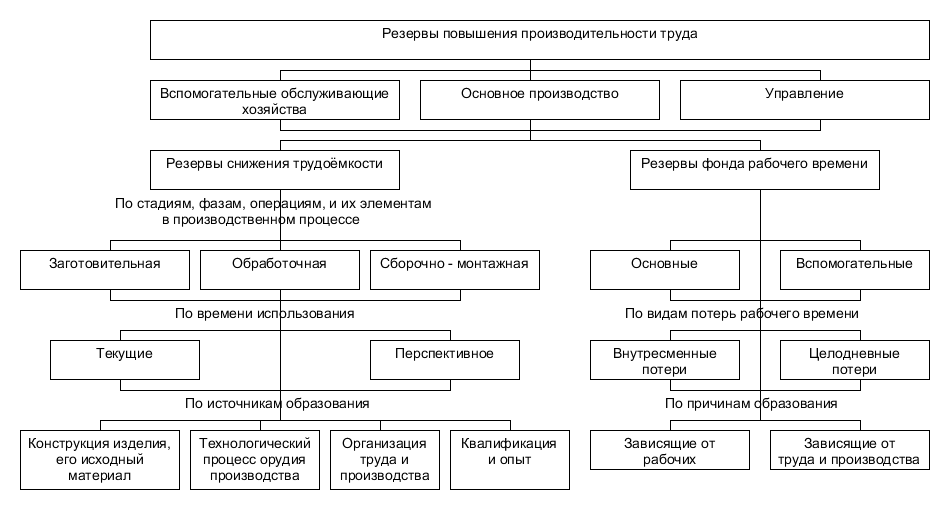
\includegraphics[width=1\linewidth]{fig/reserve1.png}}
    \caption{Резервы роста производительности труда}
    \label{ris:reserve1}
\end{figure}

Исходя из информации представленной на рисунке \ref{ris:reserve1}, можно сделать вывод, что повышение эффективности производства может быть достигнуто, как и грамотной организацией резервов рабочего времени, так и путем пересмотра техники выполнения рабочих операций, но не все резервы повышения производительности можно решить в рамках ИУС. К таким резервам относится конструктивные особенности изделия, так как требуют изменения исходной конструкции продукта, что не является задачей ИУС. 

\section{Обзор методов планирования производственных процессов.}

В данном разделе приведен перечень методов моделирования объетов и процессов.

\subsubsection{Математический}
\textbf{Описание.} Составление математического эквивалента процесса или объекта, отражающий его основные свойства.

\textbf{Область применения.} Любые процессы и объекты, поддающиеся математическому описанию.

\textbf{Достоинтсва метода.} Широкая область применения.

\textbf{Недостатки метода.} Достаточно сложно построить модель, адекватно учитывающую все факторы.

\subsubsection{Статический}
\textbf{Описание.} Модель основывается на выявленных статических закономерностях.

\textbf{Область применения.} Процессы, по которым можно собрать массив статических данных.

\textbf{Достоинтсва метода.} При наличии качественных данных метод точен и, при использовании специализированного ПО, прост в применении.

\textbf{Недостатки метода.} Большие требования к статическим данным.
\subsubsection{Экономико-математический}
\textbf{Описание.} Раздел включает в себя методы для решения экономических задач.

\textbf{Область применения.} Экономические процессы.

\textbf{Достоинтсва метода.} Метод способен моделировать экономические процессы.

\subsubsection{Имитационный}
\textbf{Описание.} Изучаемая система заменяется моделью, с достаточной точностью описывающей реальную систему, с ней проводятся эксперименты с целью получения информации.

\textbf{Область применения.} Метод используется когда дорого или невозможно использовать реальную модель и/или аналитическую модель.

\textbf{Достоинтсва метода.} Создается максимально приближенная модель, можно управлять временем системы и другими её характеристиками.

\textbf{Недостатки метода.} Сложность описания всех условий и требования вычислительной мощности.

\subsubsection{Физический}
\textbf{Описание.} Экспериментальное моделирвоание, основанное на физическом подобии уменьшенной в размерах модели.

\textbf{Область применения.} Применяется при невозможности применения аналитического метода или воспроизведения в реальном размере.

\textbf{Достоинтсва метода.} Область применения, недоступная другим методам.

\textbf{Недостатки метода.} Метод может дать надёжные результаты лишь при соблюдении физического подобия модели.

Для задач моделирования сложных, сборочных производств больше всего подходит метод имитационного моделирования, так как эксперементировать с реальным объектом экономически нецелесообразно, а также невозможно учесть все зависимости, что усложняет процесс аналитического моделирования.

\section{Обзор подходов к имитационному моделированию}

В прошлом производственные инструменты моделирования классифицировались как языки или симуляторы. \cite{Velazco} Языки были очень гибкими инструментами, но довольно сложными в использовании менеджерами и слишком трудоемкими. Симуляторы были более удобными для пользователя, но они шли с довольно жесткими шаблонами, которые недостаточно адаптировались к быстро меняющимся технологиям производства. В настоящее время доступно программное обеспечение, которое сочетает в себе гибкость и удобство для обоих, но все же некоторые авторы сообщают, что использование этого моделирования для проектирования и оптимизации производственных процессов является относительно низким. \cite{Benedettini} \cite{Holst}

Одним из наиболее часто используемых методов разработчиками производственных систем является моделирование дискретных событий. \cite{Detty} Этот тип моделирования позволяет оценить производительность системы путем статистического и вероятностного воспроизведения взаимодействий всех ее компонентов в течение определенного периода времени. В некоторых случаях моделирование производственных систем требует непрерывного подхода к моделированию. \cite{Robinson} Это те случаи, когда состояния системы постоянно меняются, как, например, при движении жидкостей на нефтеперерабатывающих или химических заводах. Поскольку непрерывное моделирование не может быть смоделировано цифровыми компьютерами, оно выполняется небольшими дискретными шагами. Это полезная функция, поскольку во многих случаях необходимо комбинировать как непрерывное, так и дискретное моделирование. Это называется гибридным моделированием \cite{inproceedings}, которое необходимо во многих отраслях, например в пищевой промышленности. \cite{Benedettini}

На данный момент существует большое количесво подходов к имитационному моделированию. Ниже приведена таблица \ref{tab:ImMethods} общих применений моделирования в производстве\cite{Jahangirian}:

% Please add the following required packages to your document preamble:
% \usepackage{graphicx}
\begin{table}[H]
    \caption{Задачи и методы моделирования производства}
    \label{tab:ImMethods}
    \centering
    \resizebox{\textwidth}{!}{%
    \begin{tabular}{|c|c|c|}
    \hline
    Задача                                                                                    & Подход                                                                                              & Описание области задачи                                                                                                                                                                                           \\ \hline
    \begin{tabular}[c]{@{}c@{}}Балансировка сборочной\\ линии\end{tabular}                    & \begin{tabular}[c]{@{}c@{}}Дискретно-событийное \\ моделирование(ДСМ)\end{tabular}                  & \begin{tabular}[c]{@{}c@{}}Проектирование и балансировка \\ сборочной линии\end{tabular}                                                                                                                          \\ \hline
    Планирование мощности                                                                     & \begin{tabular}[c]{@{}c@{}}Системная динамика(СД),\\ Метод Монте-Карло(МК),\\ ДСМ\end{tabular}      & \begin{tabular}[c]{@{}c@{}}Неопределенность из-за \\ изменения уровней мощности, \\ увеличения текущих ресурсов, \\ улучшения текущих операций \\ для увеличения мощности\end{tabular}                            \\ \hline
    Управление запасами                                                                       & ДСМ, МК                                                                                             & \begin{tabular}[c]{@{}c@{}}Стоимость имущества, \\ уровни запасов, \\ пополнение, \\ определение размеров партии\end{tabular}                                                                                     \\ \hline
    Just-in-time                                                                              & ДСМ                                                                                                 & Проектирование систем Канбан                                                                                                                                                                                      \\ \hline
    Планирование                                                                              & ДСМ                                                                                                 & \begin{tabular}[c]{@{}c@{}}Пропускная способность, \\ надежность доставки, \\ последовательность операций, \\ планирование производства, \\ минимизация времени простоя, \\ спрос, готовность заказа\end{tabular} \\ \hline
    \begin{tabular}[c]{@{}c@{}}Система управления \\ цепями поставок\end{tabular}             & \begin{tabular}[c]{@{}c@{}}ДСМ, СД, \\ Агентное моделирование\\ (АГ), Сети Петри (СП),\end{tabular} & \begin{tabular}[c]{@{}c@{}}Нестабильность в цепочке поставок, \\ системах инвентаризации / распределения\end{tabular}                                                                                             \\ \hline
    Распределение ресурсов                                                                    & ДСМ                                                                                                 & \begin{tabular}[c]{@{}c@{}}Выделение оборудования для \\ улучшения технологических процессов, \\ сырья для заводов, выбора ресурсов\end{tabular}                                                                  \\ \hline
    \begin{tabular}[c]{@{}c@{}}Планирование производства и\\ управление запасами\end{tabular} & ДСМ, АГ,                                                                                            & \begin{tabular}[c]{@{}c@{}}Страховой запас, \\ размер партии, \\ узкие места, \\ правила прогнозирования \\ и планирования\end{tabular}                                                                           \\ \hline
    Прогнозирование                                                                           & Гибридные технологии                                                                                & \begin{tabular}[c]{@{}c@{}}Сравнение разных \\ моделей прогнозирования\end{tabular}                                                                                                                               \\ \hline
    \end{tabular}%
    }
    \end{table}


    Как видно из таблицы \ref{tab:ImMethods} по результатам исследования \cite{Jahangirian} было выявлено, что наиболее используемый метод моделирования производсвенного планирования является дискретно-событийная модель. 